% MODULE 5: BEYOND NODAL DAMPING: EFFECTIVE OPERATORS. Panel box (reference px): x 405-756, y 459.5-793.5, title bar to y 485.5.
% Design v2: lettered SubHeads, one HeroBox (rank-two damping change), red NoteBox (M_eff scope), CardBox with the "one path grows, one path shrinks" illustration.
% Formulas follow plans/POSTER_PLAN.md (M5). Plot generated by figures/module5/make_m5_plot.py from the real CSV. Text edge x = 415, right edge x = 746.
\begin{scope}
  % ---------------------------------------------------------------- A: exact Schur self-energy
  \SubHead{A}{Exact Schur self-energy}{415}{495}
  \ProvedTag{722}{495}{EXACT}
  \node[anchor=west,inner sep=0pt,text=PNavy] at (415,510) {\fontsize{23pt}{25pt}\selectfont $S_r(s)=sI-A_{rr}-A_{rc}(sI-A_{cc})^{-1}A_{cr}$};
  \node[anchor=west,inner sep=0pt,text=PNavy] at (415,525) {\fontsize{24pt}{26pt}\selectfont $T(s)=s^2M+sD_0+L+\Pi(s)$};
  \node[anchor=west,inner sep=0pt,text=PMuted] at (610,525) {\FiraMed\fontsize{17.5pt}{18pt}\selectfont $r$ retained, $c$ eliminated states};

  % ---------------------------------------------------------------- B: even/odd split
  \SubHead{B}{Even/odd split $\Pi=\Pi_e+\Pi_o$}{415}{543}
  \ProposedTag{717}{543}{PROPOSED}
  \node[anchor=west,inner sep=0pt,text=PNavy] at (415,558) {\fontsize{22pt}{24pt}\selectfont $L_{\rm eff}=L+\Pi_e(0),\quad D_{\rm eff}=D_0+\Pi_o(s)/s$};
  \node[anchor=west,inner sep=0pt,text=PNavy] at (415,573) {\fontsize{22pt}{24pt}\selectfont $M_{\rm eff}=M+[\Pi_e(s)-\Pi_e(0)]/s^2$};
  \node[anchor=west,inner sep=0pt,text=PNavy] at (415,588) {\fontsize{24pt}{26pt}\selectfont $T=s^2M_{\rm eff}+sD_{\rm eff}+L_{\rm eff}$};
  \NoteBox{612}{566}{746}{599}{PRed}
  \node[anchor=west,inner sep=0pt,text=PRed,align=left,font=\FiraSemi\fontsize{17.5pt}{19pt}\selectfont] at (620,582.5) {$M_{\rm eff}$ is an operator,\\not rotor inertia.};

  % ---------------------------------------------------------------- C: damping operator + hero
  \SubHead{C}{Damping operator $D_H(\Omega)=\mathrm{Herm}\,Z(j\Omega)$}{415}{612}
  \HeroBox{415}{622}{746}{653}
  \node[inner sep=0pt,text=PNavy] at (500,637.5) {\fontsize{28pt}{30pt}\selectfont $\delta D_H=\tfrac12(a\,v^H+v\,a^H)$};
  \node[anchor=west,inner sep=0pt,text=PGreen,align=left,font=\FiraSemi\fontsize{19.5pt}{21pt}\selectfont] at (590,637.5) {one positive, one\\negative eigenvalue};

  % ---------------------------------------------------------------- plot: real 60-case signed eigenvalues of delta D_H
  % source: reports/poster/ias2026/one_mode_20261005/generated/data/TABLE_02_FINITE_DELAY_RANK_LAW.csv (lambda_min, lambda_max; 60 rows)
  \node[anchor=north west,inner sep=0pt] at (415,657) {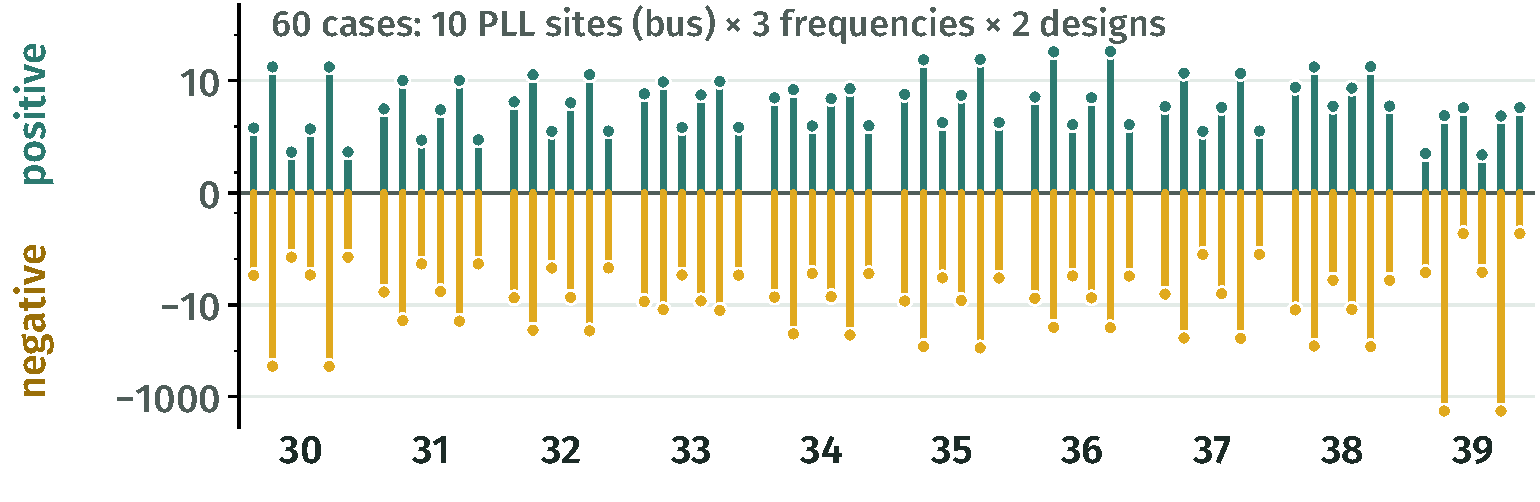
\includegraphics[width=331\PX,height=84\PY]{figures/module5/m5_signed_eigs.pdf}};
  \node[anchor=north west,inner sep=0pt,text=PMuted] at (415,742) {\parbox{331\PX}{\raggedright\FiraMed\fontsize{17.5pt}{18.5pt}\selectfont 60 cases: 10 PLL sites $\times$ 3 frequencies $\times$ 2 designs}}; % source: experiments/poster_julia_validation_20261003/RANK_LAW_SUMMARY.json (cases=60; max_relative_update_error=4.8476337614923296e-08, not printed)

  % ---------------------------------------------------------------- conclusion with illustration: damping grows along one path, shrinks along the other
  \CardBox{415}{758}{746}{790}
  \begin{scope}[line cap=round,line join=round]
    \draw[PMist,line width=1.8pt] (442,783) -- (458,764) -- (474,783) -- cycle;
    \foreach \x/\y in {442/783,458/764,474/783}{\fill[PTeal!55!PMist] (\x,\y) circle (4);}
    \draw[-{Stealth[length=6pt,width=6pt]},PTeal,line width=1.8pt] (445.5,778) -- (454.5,767.5);
    \draw[-{Stealth[length=6pt,width=6pt]},PGoldDeep,line width=1.8pt] (461.5,767.5) -- (470.5,778);
    \fill[PTeal] (431,771) circle (5.5);\fill[PGoldDeep] (485,771) circle (5.5);
    \draw[white,line width=1.8pt] (428.2,771) -- (433.8,771) (431,768.2) -- (431,773.8) (482.2,771) -- (487.8,771);
  \end{scope}
  \node[anchor=west,inner sep=0pt,text=PGreen,align=left,font=\FiraBold\fontsize{19pt}{21pt}\selectfont] at (500,774) {A local change moves damping between paths;\\damping at one frequency is no certificate.};
\end{scope}
